O presente trabalho busca propor um modelo numérico capaz de prever os perfis de
temperatura e pressão no interior de uma amostra de concreto refratário sujeito
ao aquecimento. Para tanto é fundamental o uso de experimentos para a obtenção
das propriedades necessárias ao modelo bem como ensaios que permitam a validação
do mesmo. Assim, a presente seção apresenta o levantamento das características
necessárias ao modelamento bem como os testes para validação do modelo. Além
disso no Apência A há uma seção específica (Seção \ref{codigo}) que descreve o modelo
matemático bem como a sua implementação em Python usando o pacote FEniCS. É
porém de fundamental importância determinar uma composição que será utilizada
e modelada, e portanto é a seção que inicia o presente capítulo.

\section{Composição de Concreto Refratário Aluminoso}

        
\section{Caracterização Experimental}\label{mat:exp}
As propriedades fundamentais para o modelo são

\begin{itemize}
\item Permeabilidade ($\kappa$)
\item Condutividade Térmica ($\lambda$)
\item Densidade ($\rho$)
\item Calor Específico ($\C_p$)
\item Água liberada por desidratação ($w_d$)
\end{itemize}

Além disso, as curvas de sorção isotérmica também se faz necessária, porém,
devido a ampla dificuldade em mensurá-la, o presente trabalho adotará a curva
padrão para concretos refratários reportada por Gong et al\cite{Gong1995a}. Além
de tais propriedades ensaios de Porosidade Aparente ($n_a$), e de Resistência
Mecânica também foram realizados para avaliar a suas relações com as
propriedades obtidas.

    \subsection{Porosidade e Densidade Aparente}\label{mat:porosidade}
    A porosidade e a densidade aparente dos materiais foram obtidas através do
    método de imersão usando o princípio de Arquimedes em corpos de prova
    tratados previamente a temperaturas de 30$^\circ$C, 110$^\circ$C,
    150$^\circ$C e 200$^\circ$C, 250$^\circ$C e 350$^\circ$C. Devido a
    possibilidade de hidratação do cimento, o fluído de imersão utilizado foi
    querosene (conforme recomendado pela norma ASTM C 830) e os valores de
    porosidade aparente, $n_a$ e de densidade aparente, $\rho$, foram calculados
    conforme as Equações \ref{eq:PA} e \ref{eq:DA}, respectivamente.

    \begin{equation}
      \label{eq:PA}
      n_a (\%)= 100 \ \frac{P_u-P_s}{P_u-P_i}
    \end{equation}

    \begin{equation}
      \label{eq:DA}
      \rho = \frac{P_s}{P_s - P_i} \ \rho_f
    \end{equation}

    Onde $P_u$ é o peso a úmido, $P_s$ é o peso da amostra submerso no fluído,
    $P_s$ é o peso da amostra a seco e $\rho_f$ é a densidade do fluído (no
    caso a densidade da querosene, $rho_f = 820$ Kg/m$^3$). Cada valor foi obtido
    através da média de 5 amostras distintas.
    
    \subsection{Permeabilidade}\label{mat:perm}

    A permeabilidade dos materiais é uma medida da quantidade relativa dos poros
    abertos intercomunicantes no interior de uma amostra. Para tanto, uma forma
    de medi-la é através da velocidade de um fluído dado uma determinada queda
    de pressão entre as faces de uma amostra. No presente modelo se faz
    necessário obter a permeabilidade em diferentes temperaturas e portanto
    assume-se que a microestrutura do material pode ser aproximada pelo seu
    estado após um tratamento térmico em determinada temperatura, sendo a medida
    feita em temperatura ambiente, seguindo a Norma ASTM C577. As medidas são
    obtidas pela média de 3 amostras de formato cilíndrico com raio de 35mm e
    espessura de 25mm. Para a vedação do sistema se utiliza silicone além de um
    O-ring de borracha. O esquema é apresentado na Figura \ref{fig:perm}. O
    modelo utiliza a condutividade hidráulica que é obtida a partir da constante
    de permeabilidade Darciana ($k_1$) que representa as perdas de energia
    viscosa a baixas velocidades do ar. A medida porém também permite a medição do
    parâmetro $k_2$ devido a não linearidade da velocidade, caracterizada pela
    equação de Forchheimer, \ref{eq:forch}. Este segundo parâmetro diz respeito
    a perda de energia cinética a altas velocidades.

    \begin{equation}
      \label{eq:forch}
      \frac{P_e^2 - P_s^2}{2 \ P \ L} = \frac{\mu}{k_1} \ v_s + \frac{\rho}{k_2}v_s^2
    \end{equation}

    Onde $P_e$ e $P_s$ são as pressões absolutas na entrada e na saída da
    amostra medidas em atm, $P$ é a pressão a uma determinada vazão de ar, $L$ é a
    espessura da amostra em mm, $\mu$ é a viscosidade do ar medida em Pa s,
    $\rho$ é a densidade do ar g/cm$^3$ e $v_s$ é a velocidade do fluído em
    m/s.

    
    
  \begin{figure}[ht]
	\centering
	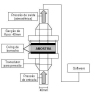
\includegraphics[width=9cm]{./figures/perm.pdf}
	\caption{Esquema de montagem do ensaio da medida de permeabilidade.  \label{fig:perm}}
  \end{figure}

   

    \subsection{Resistência Mecânica}\label{mat:rm}
    A resistência mecânica foi obtida através do ensaio de flecão em 3 pontos no
    mesmo intervalo de temperaturas usado para a obtenção da porosidade e
    densidade aparente, sendo realizados de acordo com a norma ASTM C133
    utilizando 5 corpos de prova no formato de paralelepípedos com dimensões de
    25 x 25 x 150 mm$^3$. O equipamento utilizado foi uma máquina de ensaios
    mecânicos universal (MTS, Modelo 810, USA) usando uma taxa de carregamento
    constante de 12.9 N.s$^{-1}$. O módulo de ruptura ($\sigma_f$) foi calculado
    pela Equação \ref{eq:modulo_rup}.

    \begin{equation}
      \label{eq:modulo_rup}
     \sigma_f = \frac{3 \ P \ L}{2 \ b \ d^2}
    \end{equation}

    Onde $P$, é a carga de ruptura medida em N, L é a distância  entre os
    apoios, fixa em 127 mm; b é a largura e d , a altura do corpo de prova,
    sendo todas as distâncias medidas em mm.
    
    \subsection{Termogravimetria (TGA)}\label{mat:TGA}
    
    Um dos principais ensaios para a simulação do processo de explosão durante o
    processo de secagem em escala laboratorial é o ensaio de termogravimetria. O
    sistema consiste em um forno com uma balança acoplada onde se mede a
    temperatura da amostra e do forno além da evolução do peso de uma amostra
    cilíndrica com 40 mm de diâmetro e 40 mm de altura. Os corpos são aquecidos
    após cura a 30$^\circ$C por 24 horas. Foram utilizadas taxas de aquecimento
    constantes de 2$^\circ$C.min$^{-1}$, 5$^\circ$C.min$^{-1}$ e
    20$^\circ$C.min$^{-1}$ no intervalo de 30$^\circ$C e 800$^\circ$C. A perda
    de massa e sua taxa temporal foram obtidas através das Equações
    \ref{eq:TGA_W} e \ref{eq:TGA_DTG}.

    \begin{equation}
      \label{eq:TGA_W}
      W = \left( \frac{M_0-M}{M_0-M_f} \right) \ 100
    \end{equation}

    \begin{equation}
      \label{eq:TGA_DTG}
      DTG = \frac{\partial W}{\partial t}
    \end{equation}

    Onde $M_0$ é a massa inicial da amostra, $M$ é a massa observada num
instante t, e $M_f$ corresponde à massa final da amostra (todas medidas em
gramas). $W$ é a perda de massa percentual, enquanto DTG é a taxa de perda de
massa (medida em \%.min$^{-1}$). A Figura \ref{fig:TGA} apresenta o esquema de
montagem do ensaio de termogravimetria.
    
 \begin{figure}[ht]
	\centering
	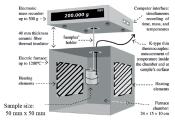
\includegraphics[width=9cm]{./figures/TGA.pdf}
	\caption{Esquema de montagem do ensaio de termogravimetria.  \label{fig:TGA}}
  \end{figure}



    \subsection{Condutividade Térmica e Calor Específico}\label{mat:condutividade}
    A condutividade térmica é obtida através do método do fio quente (com a
    configuração dos fios paralelos) através do
    equipamento Netzsch TCT 426. A medição se dá em um sistema de 3 tijolos com
    mesma composição dispostos um sobre os outros. Entalhes de 0.4mm são
    realizados nos tijolos usando uma retífica modelo Ferdimat T42 a fim de
    acomodar os fios do termopar.

    A técnica obtém o valor de condutividade através de uma estimativa baseada
    no tempo em que o calor gerado pelo fio quente (FQ) devido ao efeito Joule leva
    para ser percebido no termopar da amostra ($T_a$) em uma condição de equilíbrio
    térmico entra o conjunto de tijolos e o forno (através da medida de um
    termopar de referência $T_r$). Tal ensaio permite a obtenção do calor
    específico através da medida de difusividade térmica do material. A Figura \ref{fig:fio_quente}
    apresenta o {\it layout} do ensaio.

  \begin{figure}[ht]
	\centering
	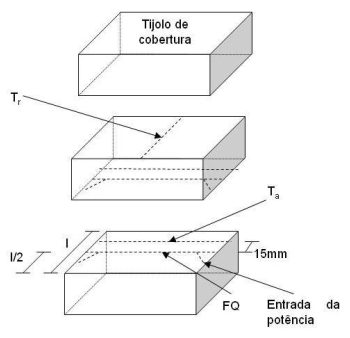
\includegraphics[width=9cm]{./figures/fio_quente.pdf}
	\caption{Esquema de montagem do ensaio da técnica de fio quente para obtenção
    da condutividade térmica e calor específico.  \label{fig:fio_quente}}
  \end{figure}


    
%%% Local Variables:
%%% mode: latex
%%% TeX-command-extra-options: "-shell-escape"
%%% TeX-master: "TCC-Secagem"
%%% End:
